\externaldocument{capitulo04}

\chapter{\hspace*{3pt} POR: Processo Objeto - Representação}
\label{chap:por}

A literatura demonstra, que a racionalização do conhecimento é uma área fértil para perspectivas e abordagens distintas. No entanto acreditamos que no âmbito da elaboração de modelos conceituais, uma maneira de representar o conhecimento, perceber os pontos de convergência entre essas teorias pode fornecer um ponto de apoio no processo de representação conceitual acerca de um determinado domínio.

Neste propósito, defendemos que é preciso um processo que seja capaz guiar os modeladores através dos pontos de convergência de maior destaque. Evidenciar a discussão inerente ao processo de construção de modelos conceituais, passando de maneira ativa por cada uma das etapas identificadas e discutidas nas abordagens que servem de fundamentação para este trabalho.

Com base nas teorias apresentadas neste trabalho, elaboramos um fluxo que visa auxiliar a elaboração de modelos conceituais. O processo proposto contempla fases que possuem como propósito guiar o modelador na busca acerca do seus conhecimentos sobre o contexto e como sucedeu sua aquisição. Tal busca, intencional refletir na sua representação mais expressiva e completa.

Este processo, embora esteja dividido em três fases (Percepção, Racionalização e Representação), apresenta sua discussão centrada na fase dois, a racionalização, pois entendemos que esta fase contém o ponto crítico do processo de raciocínio e representação do conhecimento. Em cada fase, identificamos uma ou mais etapas que irão compor o fluxo, que serão apresentadas nas seções seguintes.

A figura \ref{fig:por-resumido} representa essas etapas resumidamente.
\begin{figure}
    \centering
    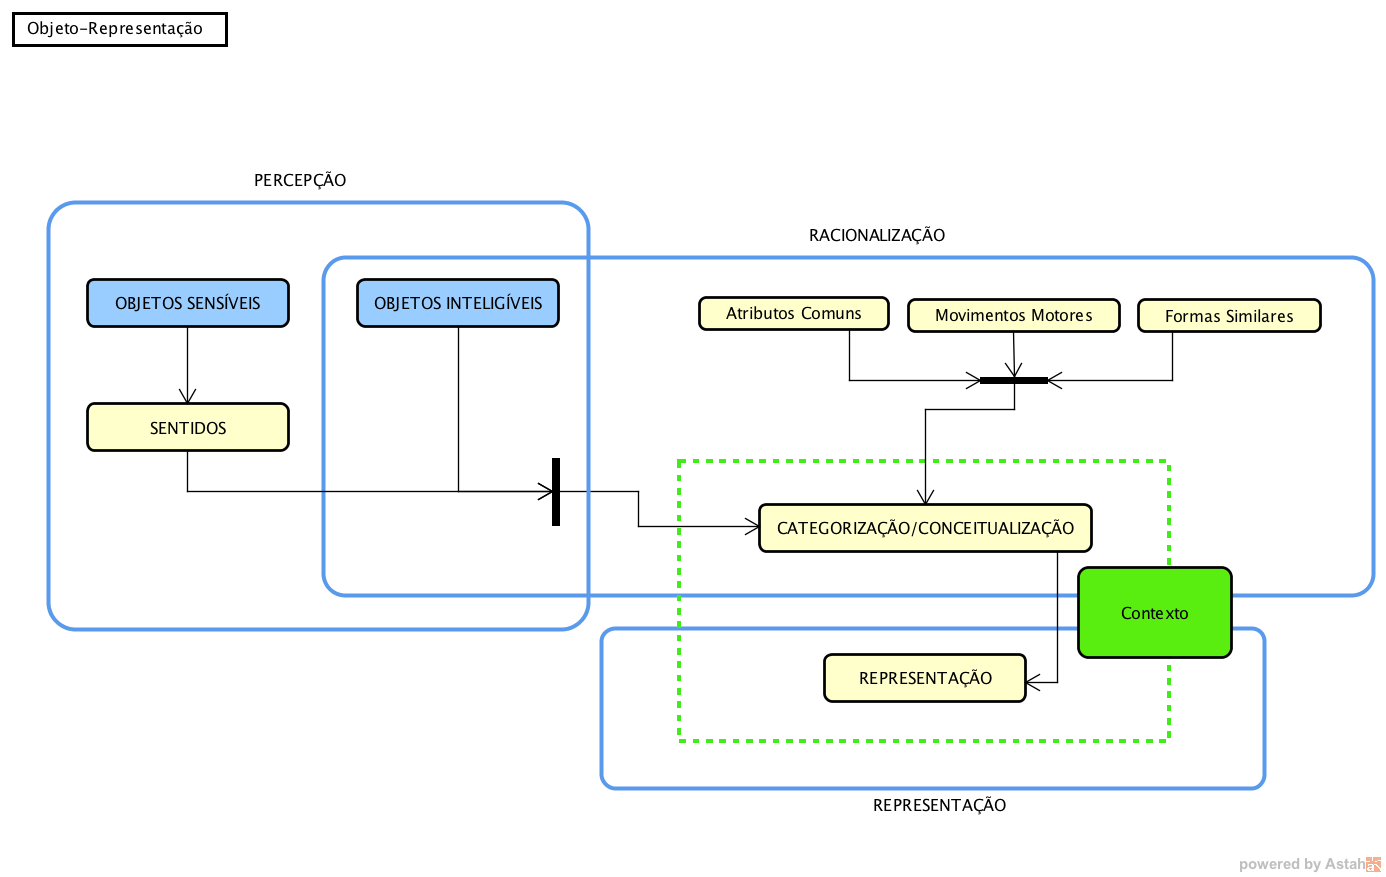
\includegraphics[width=\textwidth]{imagens/Fases_Processo_O-R.png}
    \caption{Fases do Processo Objeto-Representação}
    \label{fig:por-resumido}
\end{figure}

\section{\hspace*{3pt} Fase 01: Percepção}
\label{sec:percepcao}

A fase um foi definida como a Percepção, cuja função é fornececer os objetos que serão racionalizados. 

Objeto é tudo aquilo que nos circunda ou é designado pelo homem; são as ``coisas" do mundo. Nesta dissertação, o termo ``objeto” é empregado de maneira ampla e pode representar tanto objetos concretos (ex.: um animal ou um veículo), quanto objetos abstratos (ex.: um departamento ou um dragão) \citep{dahlberg:1978.teoria, machado:2009.projeto}. 

Podemos, ainda, categorizá-los em objetos sensíveis, isto é, aqueles objetos que são evidenciados para nós através de um, ou mais, sentidos e objetos inteligíveis, cuja sensação é fruto de um processo mental, como por exemplo a junção de ideias de mulher e peixe, para formar uma sereia ou conceitos que não existem de maneira física, como sentimentos. 

Ao categorizar os objetos em sensíveis e inteligíveis, apesar de reconhecer toda a batalha filosófica travada ao longo dos séculos entre as correntes denominadas Empirismo, Racionalismo e Criticismo, não estamos assumindo uma postura Empirista, mas queremos apenas evidenciar os objetos abstratos, como fruto um processo racional e reflexivo, a despeito de quaisquer discussões filosóficas subjacentes. 

A base da percepção humana são os sentidos, sendo estes estimulados de maneira contínua por um fluxo de acontecimentos. Disto resulta uma excitação neural chamada de sensação \citep{alexandre:2007.factores}.

Sensação, segundo o dicionário online \citet{priberam:2015} é ``a impressão produzida pelos objetos exteriores num órgão dos sentidos, transmitida ao cérebro pelos nervos, onde se converte em ideia, julgamento ou percepção''.

Na introdução da Crítica da Razão Pura, \citet{kant:1983.critica} afirma que: 

\begin{quote}
``Não há dúvida de que todo o nosso conhecimento começa com a experiência; do contrário, por meio do que a faculdade de conhecimento deveria ser despertada para o exercício senão através de objetos que toquem nossos sentidos e em parte produzem por si próprios representações, em parte põem em movimento a atividade do nosso entendimento para compará-las, conectá-las ou separá-las e, desse modo, assimilar a matéria bruta das impressões sensíveis a um conhecimento dos objetos que se chama experiência? […]" \citep[p.23]{kant:1983.critica}.
\end{quote}
 
Estas impressões, no entanto, são percepcionadas no espaço e no tempo, uma vez que formas puras (vazias) fazem parte das estruturas cognitivas inatas do sujeito. Elas são a condição indispensável para que possamos ter acesso ao conhecimento, isto é, a sensibilidade se expressa em duas formas: espaço e tempo, os  quais, nas palavras de \citet{kant:1983.critica}, são definidos, respectivamente, como:

\begin{quote}
``O espaço não é um conceito empírico abstraído de experiências externas. Pois a representação de espaço já tem que estar subjacente para certas sensações se referirem a algo fora de mim […] O espaço é uma representação a priori necessária que subjaz a todas as intuições externas. […] O espaço não é um conceito discursivo ou, como se diz, um conceito universal de relações das coisas em geral, mas sim uma intuição pura. […] O espaço é representado como uma magnitude infinita dada. […] A representação originária do espaço é, portanto, intuição a priori e não conceito" \citep[p.41]{kant:1983.critica}.
\end{quote}

\begin{quote}
``O tempo não é um conceito empírico abstraído de qualquer experiência. […] O tempo é uma representação necessária subjacente a todas intuições. […] Sobre essa necessidade a priori também se funda a possibilidade de princípios apodíticos das relações do tempo, ou de axiomas do tempo em geral. […] O tempo não é um conceito discursivo ou, como se diz, um conceito universal, mas uma forma pura da intuição sensível. […] A infinitude do tempo nada mais significa que toda magnitude determinada do tempo só é possível mediante limitações de um tempo uno subjacente" \citep[p.44--45]{kant:1983.critica}. 
\end{quote}

O espaço e o tempo não são conceitos, visto que não são elaborados pelo sujeito tendo como ponto de partida suas experiências; eles simplesmente existem no sujeito cognoscente, que ao conhecer os objetos do mundo, o fazem de um modo dimensionado e associado à ideia de movimento, de mudança, de evolução, ou mesmo em estágios ou locais diferentes. Por isso as noções de espaço e de tempo são condições necessárias para o conhecimento dos objetos do mundo.

É através de sua percepção que um indivíduo organiza e interpreta suas impressões sensoriais para atribuir significado ao seu meio. Do ponto de vista cognitivo, a percepção envolve processos mentais que interpretam os dados oriundos dos sentidos e os associam aos conceitos.

\section{\hspace*{3pt} Fase 02: Racionalização}
\label{sec:racionalizacao}

A racionalização quem nos permite dar significados aos estímulos que recebemos, transformando os dados oriundos das percepções em ideias ou conceitos.

Esta fase compartilha a visão atomística, que defende que a compreensão de um objeto implica o reconhecimento das partes para ter o entendimento do todo. Embora a visão holística - aquela que defende que a interpretação de um objeto se dá pelo todo - seja reconhecida, o todo quando inserido em um contexto, pode apresentar características que não sejam relevantes para a conceitualização do objeto.

Os experimentos propostos por \citet{rosch:1999.principles}, para encontrar o nível médio de abstração: atributos comuns, movimentos motores, forma objetiva e semelhança da forma, ou as forma de conhecer o mundo, quando dentro do contexto, permitem que identifiquemos quais características que são importantes para definição do objeto. 

O contexto delimita no universo do nosso discurso, qual as características dos objetos que percebemos fazem sentidos, e precisam ser compartilhadas para que nossas representações façam sentido para nossos interlocutores.  

A categorização reflete a nossa capacidade para agrupar entidades únicas em conjuntos, usando como regras de agrupamento as características que compartilham entre si. 

\subsection{\hspace*{3pt} Formas de Conhecer o Mundo}

Atributos comuns são as características que dois ou mais objetos de uma mesma categoria compartilham. Ex.: ter bicos, ter penas, por ovos.

Movimentos motores representam a maneira como interagimos determinados objetos, os movimentos musculares associados à utilização do objeto. Ex.: o ato de sentar em uma cadeira ou de cortar com um serrote.

Formas Objetivas e Similares dizem respeito a forma como o objeto se apresenta, isto é, a forma que ele possui. Ex.: cadeira de jantar, cadeira de praia, poltrona.

Nossa experiência associa características novas àquelas percebidas previamente, que sejam semelhantes. Refletir acerca da maneira como as características nos chegam nos ajudam entender como estamos categorizando um determinado grupo de características

\subsection{\hspace*{3pt} Contexto}

É o contexto que define o universo do discurso, influencia os conceitos que serão utilizados para expressarem um grupo de objetos ou relações. ``A relevância do contexto para a nossa capacidade de interpretar o que percebemos não é uma fantasia filosófica acadêmica esotérica. É o que fazemos todos os dias (Olson, 2012)''. Ex.: Podemos falar de cinema, enquanto empresas de exibição de filmes de cinema; ou de cinema do ponto de vista da indústria que produz imagens com impressão de movimento, contendo narrativa.

Podemos afirmar então, que o ato de categorizar passa a ser encarado como um processo interacional, construído de maneira discursiva e dependente de um contexto \citep{carvalho:2013.categorizacao}.

\citet{vickery:1980.classificacao}, citado por \citet{silva:2011.categorias}, reforçando essa ideia diz: 

\begin{quote}
``A aquisição do conhecimento é um processo ativo. É uma interação concreta entre o organismo humano e seu ambiente, no curso do qual o ambiente é física e objetivamente mudado, e o organismo é também mudado, mas mental e subjetivamente. Estudando o desenvolvimento das categorias conceituais, não são apenas as atividades mentais como ‘a distinção’ que devem ser levadas em consideração. A atividade total, mental e física é envolvida." (\citealp[p.236]{vickery:1980.classificacao} \textit{apud} \citealp{silva:2011.categorias})
\end{quote}

\citet[p.104]{medrado:2008.espelho}, afirma que o contexto trás além dos aspectos linguísticos, elementos corporais, gestuais, identidades institucionais e papéis sociais, ou seja, elementos socioculturais, produzindo uma relação dinâmica entre linguagem, cognição e interação \citep{carvalho:2013.categorizacao}.

\subsection{\hspace*{3pt} Categorização}

Uma das formas que a categorização pode se dar, segundo \citet{richardson:1985.pesquisa}, é como o resultado da classificação progressiva dos elementos. A maior parte deste processo de categorização ocorre automática e inconscientemente, este processo só se torna perceptível a nós quando ocorrem casos dúbios. Oferecemos uma maneira de pensar sobre os conceitos e construir gradualmente o sistema de categorias que irão comportar os conceitos, conscientemente.

O significado linguístico, está estreitamente relacionado com os processos de categorização, ``os conceitos, os significados não são, pois, rótulos das coisas nem objetos mentais aprioristicamente dados, mas categorias e, como tal, criações da cognição humana que servem para dar sentido ao mundo” \citep[p. 298]{da:2006.mundo}

Categorizar é agrupar entidades (objetos, ideias, ações, etc) por semelhança \citep{lima:2007.categorizacao}. Este é um processo mental habitual ao homem, pois vivemos automaticamente classificando ideias e coisas a fim de compreender e conhecer a realidade \cite{piedade:1983.introducao}.

A Figura \ref{fig:por-estendido}, desdobra a fase de Categorização/Conceitualização.

\begin{figure}
    \centering
    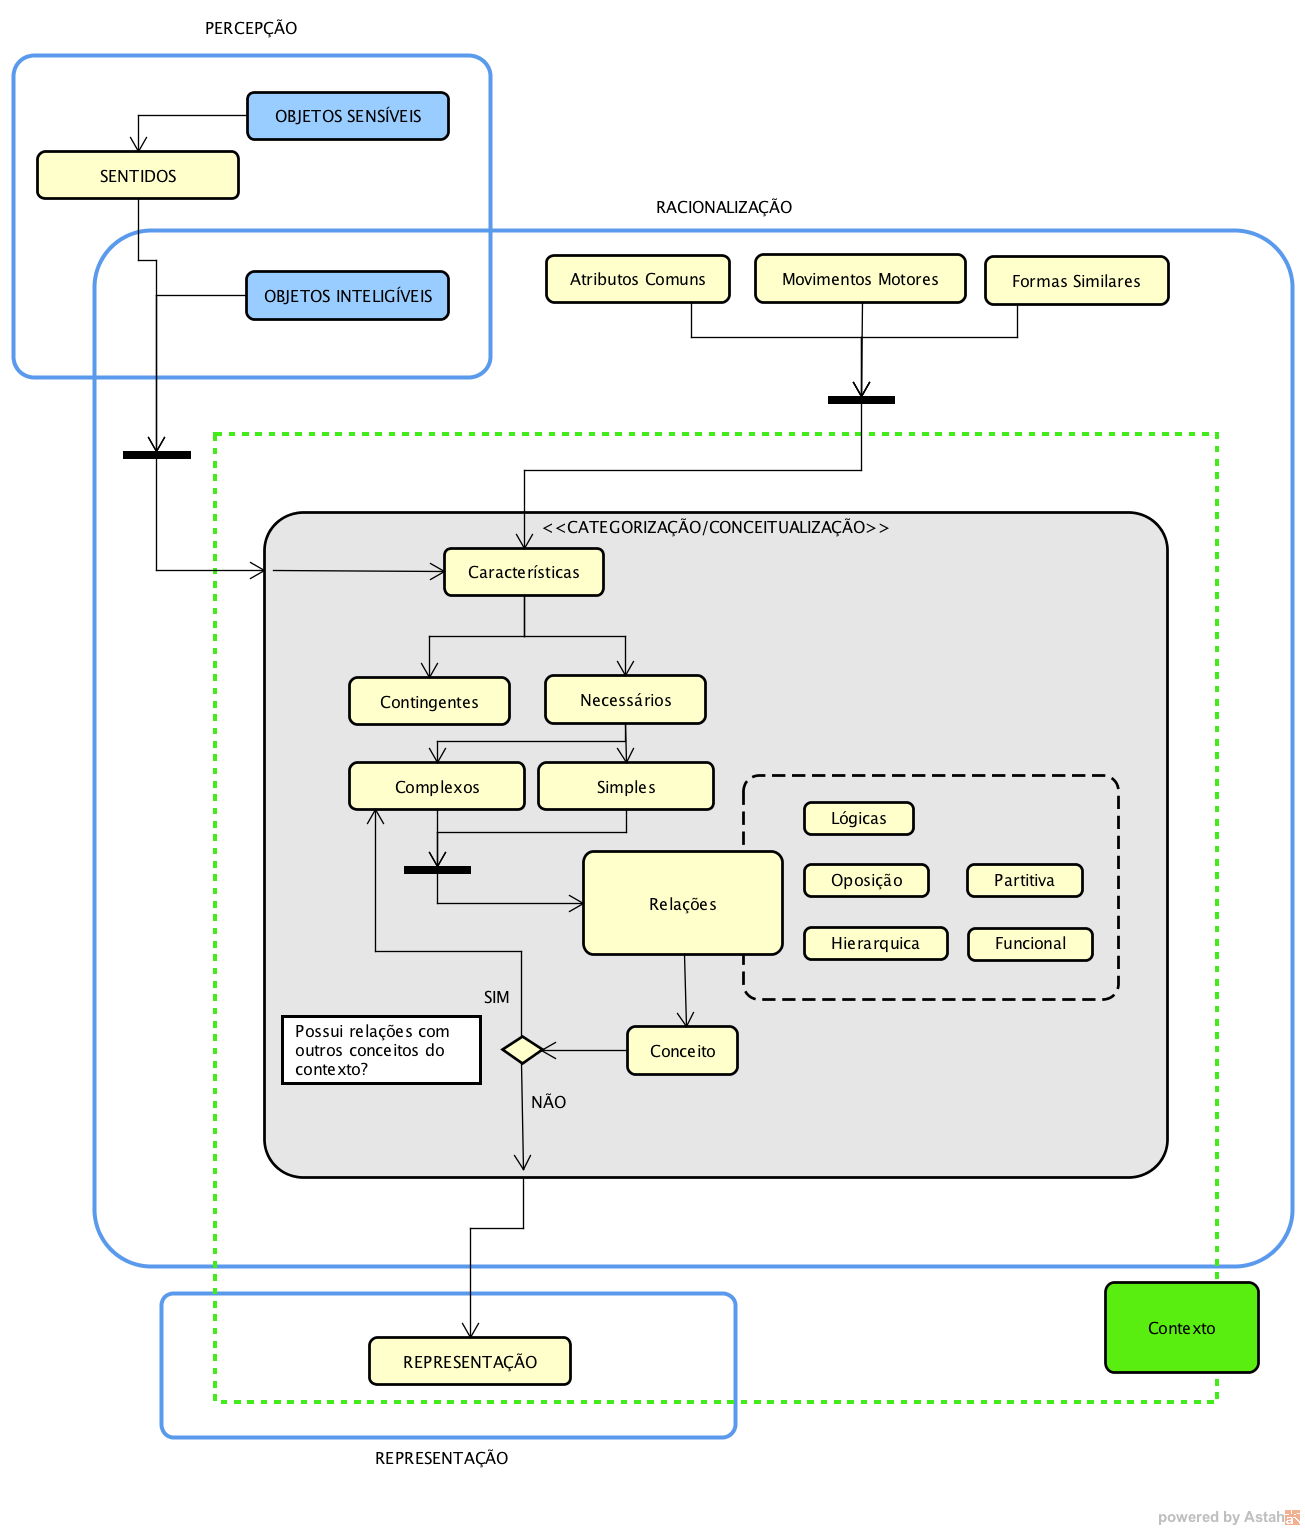
\includegraphics[width=\textwidth]{imagens/Processo_O-R_Estendido_2.png}
    \caption{Processo Objeto-Representação - Fluxo Estendido}
    \label{fig:por-estendido}
\end{figure}

\subsubsection{\hspace*{3pt} Características}

\citet{dahlberg:1978.teoria} define característica, como uma unidade de conhecimento. Cada conceito, é então entendido como um conjunto de características necessárias para a sua definição, e cada característica pode ser definida como um enunciado verdadeiro acerca do objeto \citep{dahlberg:1978.fundamentos}

Enunciado é qualquer frase ou oração, que exprima um pensamento de sentido completo, isto é, àquele pensamento que admite apenas um dos valores verdadeiro ( v ) ou falso ( f ). Mas para nossos propósitos, consideraremos apenas as frases declarativas cujo valor de verdade possa ser asseguradamente o verdadeiro (v). 

Pelo fato de os enunciados sobre um objeto serem tão vastos, quanto nossos conhecimentos permitam, podemos tomar como exemplo a tabela categorial de Aristóteles, afim de permitir a identificação do maior número de características possíveis.

As categorias Aristotélicas, apresentadas na Tabela \ref{tab:categorias}, foram escolhidas como base neste trabalho, primeiro por entender a importância de sua classificação categórica para as teorias subjacentes e segundo por seguir a proposta de \citep{dahlberg:1978.fundamentos}. 

\begin{table}
\centering
\resizebox{\textwidth}{!}{%
\begin{tabular}{|>{\centering\arraybackslash}m{6cm} 
				|>{\centering\arraybackslash}m{6cm}
                |>{\centering\arraybackslash}m{6cm}|}
\hline
		Categoria &
        Descrição &
        Exemplo \\
\hline
		Matéria & 
        É o que existe em si mesmo, o próprio objeto e seu material de origem. & 
        de pedra, de madeira, de vidro, etc. \\ 
\hline
		Qualidade & 
        É a determinação da matéria da substância, atribuindo-lhe partes distintas de outras partes. &
        possuir determinada estrutura, determinada forma, ser redondo, denso, colorido etc. \\
\hline
		Quantidade (Extensão) &
		É a determinação da natureza ou da forma da substância. &
        possuir comprimento, largura, peso etc. \\
\hline
		Relação &
        É a referência que um objeto ou uma característica possui com uma outra. &
        ser o dobro, ser mais largo, ser causa de, ser condição de, etc. \\
\hline
		Processo (atividade, ação) &
        É o exercício das faculdades ou de poder sobre o objeto, de modo a produzir um efeito em alguma outra coisa ou nele mesma. &
        começar, continuar,  terminar, realizar algo etc. \\
\hline
		Modo de ser &
		É posição relativa que as partes de uma conceito têm quanto às outras. &
        estar em pé, sentado, voando, etc. \\
\hline
		Passividade (paixão) &
        É a recepção sofrida, por uma conceito, de um efeito produzido por algum agente. &
		ser cortado, pressionado, etc. \\
\hline
		Posse (hábito) &
        Consiste em roupas, ornamentos ou outras posses. &
        usa sapatos, está armado, etc. \\
\hline
		Localização (lugar, espaço) &
        É posição em relação aos corpos que circundam uma substância, que mede e determina o seu lugar. &
        estar em Brasília, no Rio de Janeiro, etc. \\
\hline
		Tempo &
        É posição em relação ao curso de eventos extrínsecos, e que mede a duração de uma substância. &
        em fevereiro de 1978, etc.\\
\hline
\end{tabular}
}
\caption{Categorias de Aristóteles. Fonte: \citet{dahlberg:1978.teoria}, adaptado pelo autor.}
\label{tab:categorias}
\end{table}

A emissão de enunciados utilizando a tabela das categorias, objetiva clarificar características que de outra maneira poderiam passar desapercebidas e evidencia, com maior facilidade, características simples. Sua utilização, no entanto, não tem a intenção de ser um fator limitante ou definitivo para a enunciação das características.

As formas de conhecer, propostas em \citep{rosch:1999.principles}, justificam a apreensão do conhecimento para cada uma dos enunciados acerca das categorias, de maneira que é possível relacionar cada categoria a pelo menos uma forma de conhecer, conforme Tabela \ref{tab:categorias_formas}. 

\begin{table}
\centering
\resizebox{\textwidth}{!}{%
\begin{tabular}{|>{\centering\arraybackslash}m{6cm} 
				|>{\centering\arraybackslash}m{6cm}
                |>{\centering\arraybackslash}m{6cm}|}
\hline
		{\bf Atributos Comuns} &
        {\bf Movimentos Motores} &
        {\bf Formas Similares} \\
\hline
		Qualidade &
		Qualidade &
		Qualidade \\
\hline
		Quantidade &
		Quantidade &
		Quantidade \\
\hline
		&
		&
        Relação \\
\hline
		&
		Processo &
		\\
\hline
		&
		Modo de Ser &
		\\
\hline
		&
		Passividade &
		\\
\hline
		&
		Posse &
		Posse \\
\hline
		Localização &
		Localização &
		Localização \\
\hline
		Tempo &
		Tempo &
		Tempo \\
\hline
\end{tabular}
}
\caption{Modos de Percepção do mundo x Categorias Aristotélicas. Fonte: autor.}
\label{tab:categorias_formas}
\end{table}

Os enunciados podem conter características essenciais ou acidentais. \citet{dahlberg:1978.teoria}, define as características essenciais, como aquelas que definem o próprio conceito, por isso necessárias, e acidentais aquelas que cuja a remoção não afetariam a categorização do objeto, por isso contingente.

Neste sentido, o contexto tem um papel importante, delimitando quais enunciados são essenciais para um determinado conceito. Embora a importância das características acidentais não sejam ignoradas, assim como \citet{medrado:2008.espelho}, consideraremos que apenas os enunciados necessários serão listados, quando o objeto está inserido no contexto.

Para evidenciar esse ponto, consideremos um carro (o objeto), que necessita de reparos elétricos (o contexto). Para este contexto, é irrelevante saber o tipo de combustível que o carro utiliza ou quantos quilômetros este mesmo carro é capaz rodar com um litro de gasolina.

As características, podem ainda ser simples ou complexas. Características simples dizem respeito a um único atributo. Ex.: azul, quadrado. Enquanto as complexas, usualmente, apresentam duas propriedades, ou mais, com alguma relação entre si. Ex.: pintado com tinta azul, moldado na forma quadrada. Em ambos os casos uma relação de processo \citep{dahlberg:1978.teoria}.

\subsubsection{\hspace*{3pt} Relações}

\citet{campos:2004.modelizacao}, ressalta a importância das relações entre os objetos em um dado contexto, alegando que estas relações formam as estruturas conceituais deste contexto e que as mesmas possuem natureza diversa. Seguindo a definição de \citet{dahlberg:1978.fundamentos, dahlberg:1978.teoria} para definição de conceitos, temos também a possibilidade de verificar as relações existentes entre as características de um conceito. Com esse propósito, ela define:

\begin{quote}
``Devemos estabelecer, desde logo, distinção entre as relações formais e as relações materiais, sendo que as primeiras se baseiam na comparação das características, tornando-se particularmente importantes quando se trata da compatibilidade dos conceitos e dos respectivos sistemas. As segundas têm por base o conteúdo das mesmas características. (Em síntese, deve ficar claro que as características são também conceitos, mas apenas em relação aos conceitos de que se tornaram elementos é que assumem o papel de características de conceitos)." \citep[p.14]{dahlberg:1978.fundamentos}
\end{quote}
 
\citet{machado:2009.projeto} definem relacionamento como o fato, o acontecimento que une dois, ou mais, objetos do mundo real. As características atribuídas a diferentes conceitos nos guiará a uma análise acerca das relações entre estes conceitos.

A tabela \ref{tab:dahlberg_logica}, apresentada em \citet{dahlberg:1978.teoria}, mostra os tipos de relacionamentos lógicos, através dos quais podemos definir as relações entre as características comuns. E através dos quais é possível estabelecer comparações entre os conceitos de modos a organizá-los. 

\begin{table}
\centering
\resizebox{\textwidth}{!}{%
\begin{tabular}{|>{\centering\arraybackslash}m{6cm} 
				|>{\centering\arraybackslash}m{6cm}
                |>{\centering\arraybackslash}m{6cm}|}
\hline
		Relacionamento &
        Exemplo &
        Descrição \\
\hline
		Identidade &
		A (x,x,x) e B (x,x,x) &
		As características são as mesmas;\\
\hline        
		Implicação &
		A (x,x) e B (x,x,x) &
		O conceito A está contido no conceito B; \\
\hline        
		Interseção &
		A (x,x,o) e B (x,o,o) &
		Os dois conceitos coincidem algum elemento; \\
\hline        
		Disjunção &
		A (x,x,x) e B (o,o,o) &
		Os conceitos se excluem mutuamente. Nenhuma característica em comum; \\
\hline        
		Negação &
		A (x,x,o) e B (o,x,o) &
		O conceito A inclui uma característica cuja negação se encontra em B. \\
\hline
\end{tabular}
}
\caption{Relacionamentos Lógicos. Fonte: \cite{dahlberg:1978.teoria}}
\label{tab:dahlberg_logica}
\end{table}

As relações lógicas desempenham um papel importante à medida que auxiliam a estabelecer comparações entre os conceitos, de modo a organizá-los nos seguintes relacionamentos semânticos: Relação de Hierarquia, Relação Partitiva, Relação de Oposição e Relação Funcional.

\textbf{Relação Hierárquica} (implicação) objetos que possuem características idênticas, porém um permite a ideia de um conceito mais geral que outro, então entre eles se estabelece a relação hierárquica ou relação de gênero e espécie. Pode-se então falar de conceitos mais amplos ou mais restritos. Pode-se também falar de conceito superior e inferior. O conceito superior é o mais genérico e o inferior é o mais específico \citep{dahlberg:1978.fundamentos}.
Ex.: Mamífero - Cão - Pastor-Alemão

Relações hierárquicas, podem ser estabelecidas entre conceitos específicos do mesmo gênero, e recebem o nome de relações coordenadas, ou relações horizontais.
Ex.: Cão - Cão de Pequeno Porte - Pinscher, Chihuahua, Basset \\
     Cão - Cão de Grande Porte - Fila, Labrador, Dálmata

\textbf{Relação Partitiva} existe entre dois ou mais conceitos, sendo um deles constituído por um outro. A observação de como um objeto se constitui, isto é, quais são suas partes \citep{campos:2001.organizacao}.
Ex.:: árvore- raízes, tronco, galhos, folhas, flores, frutos.

\textbf{Relação de Oposição} (negação) podem ser das seguintes espécies:
Contradição. Ex.: numérico - não numérico, presente - ausente\\
Contrariedade. Ex.: branco - preto

\textbf{Relação Funcional} (intersecção) estas relações aparecem quase exclusivamente na dependência do conceito de processo, ou seja, quando do conceito de processo deriva uma função a ele inerente. Ex.: Pintura (tem como consequência a existência de) quadros (que, por sua vez, supõe um) pintor (assim como de) críticos de arte (ou mesmo de) compradores de quadros etc.

Será fácil verificar que as relações hierárquicas e as relações partitivas se aplicam principalmente a conceitos que expressam objetos. As relações de oposição se aplicam principalmente a conceitos que expressam características. E as relações funcionais se aplicam sobretudo a conceitos que expressam processos \citep{dahlberg:1978.teoria}.

\subsubsection{\hspace*{3pt} Conceito}

Antes de mesmo da nossa capacidade da fala e da linguagem, já possuíamos a capacidade de atribuir significado às coisas. O conceito, desta forma, antecede a representação (\citealp{edelman:1995.biologia} \textit{apud} \citealp{lacerda:2012.linguagem})

A formação do conceito dar-se-á em dois níveis, no nível individual onde as características são analisadas para que se defina o tipo de relações que mantém entre si, e no nível contextual, onde um conceito é comparado com outro, então partindo de suas relações, sua correta intensão ou extensão seja definida, evidenciando o conceito mais adequado para representar.

Tomemos como exemplo um carro. Possivelmente a palavra escolhida para representar o conceito, por si só trouxe uma significância relevante. Porém listar as características deste único carro poderia ser uma tarefa extenuante e improfícua. Extenuante pois o número de enunciados que poderia proferir são inúmeros, e improfícuo porque sem determinar o contexto, esses enunciados podem não ter relevância. Desta forma, definiremos o contexto como sendo o de uma locadora de veículos.

Dentro deste contexto, considerando a atividade circunstancial de locar um carro, nosso escopo de características fica mais acessível. Onde podemos enunciar: seu modelo, cor, tipo de câmbio, quantidade de passageiros, tipo de combustível, tamanho da mala, quilometragem por litro, valor, se é aluguel por quilometro rodado ou por dia, valor do seguro, etc. Apenas para citar algumas características.

A comparação do conceito carro com outros conceitos, talvez demonstre que na verdade seja melhor representar um veículo, ou ainda que esse conceito se relacionará com o funcionário e com o locatário, e que o funcionário talvez seja alguém mais especifico.

\section{\hspace*{3pt} Fase 03: Representação}
\label{sec:representacao}

A última etapa, a representação é a forma como escolhemos exteriorizar o conceito racionalizado. Usualmente essa forma de expressão é a linguagem e a escrita, mas não se limitam apenas e elas. 

A representação do conceito em uma linguagem que seja capaz transmitir toda a sua carga de conhecimento é importante para que haja a correta representação do contexto e todo o conhecimento associado a ele. 

A forma simbólica escolhida não faz parte das análises deste trabalho, mas entendemos que as fases anteriores, a fase dois em especial, por levar ao conceito mais representativo para o contexto analisado, permitirá que  linguagens com boas regras de formalização, que permita a representação das unidades e suas relações poderá ser utilizada.